\documentclass[border=5pt]{standalone}

\usepackage{tikz}
\usepackage{xcolor}

\definecolor{vblack}{HTML}{1A1A1A}
\definecolor{vgray}{HTML}{686868}
\definecolor{vblue}{HTML}{007acc}

\begin{document}	
	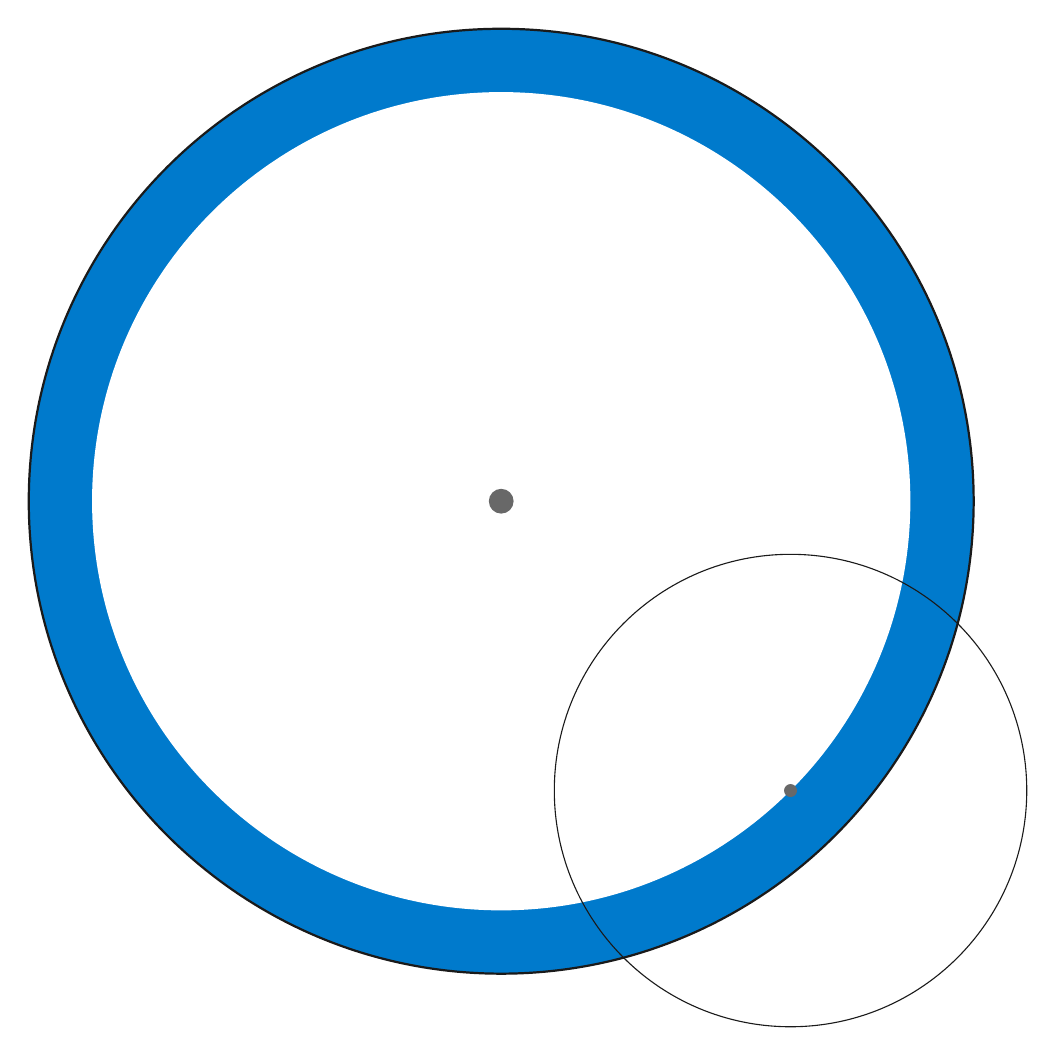
\begin{tikzpicture}
		% circles-3
		\draw[thick, draw = vblack, fill = vblue] (0,0) circle (3*2);
		\draw[fill = white, draw = none] (0,0) circle (3*1.73205);
		\draw[draw = vblack] (3*1.22475,3*-1.22475) circle (3*1);
		\draw[color = vgray, fill = vgray] (0,0) circle (3*.05);
		\draw[color = vgray, draw = vgray, fill = vgray] (3*1.22475,3*-1.22475) circle (3*0.025);
	\end{tikzpicture}
\end{document}

\begin{tikzpicture}
	% circles-1
	\draw[thick, draw = vblack] (0,0) circle (3*2);
	\draw[color = vgray, draw = vgray, fill = vgray] (0,0) circle (3*0.05) -- (3*1.28844,3*1.5296) node[midway, below right = 0pt]{$2R$};
	\draw[draw = vblack] (3*1.22475,3*-1.22475) circle (3*1);
	\draw[color = vgray, draw = vgray, fill = vgray] (3*1.22475,3*-1.22475) circle (3*0.025) node[above left = 4pt]{$50\%$} -- (3*1.22475,3*-2.22475) node[midway, right = 0pt]{$R$};
	\draw[color = vgray, dashed] (3*.517638,3*-1.93185) -- (3*1.93185,3*-.517638);
	\draw[draw = vblack] (3 * -1.93185, 3 * -.51764) circle (3 * 1);
	\draw[color = vgray, draw = vgray, fill = vgray] (3 * -1.93185, 3 * -.51764) circle (3 * .025);
	\draw[color = vgray, dashed] (3*-1.94097,3*0.48232) -- (3*-1.43977,3*-1.38819) node[midway, right = 4pt]{$<50\%$};
	\draw[draw = vblack] (3 * -.38823, 3 * 1.44889) circle (3 * 1);
	\draw[color = vgray, draw = vgray, fill = vgray] (3 * -.38823, 3 * 1.44889) circle (3 * .025);	
	\draw[color = vgray, dashed] (3*-1.38819,3*1.43977) -- (3*0.48232,3*1.94097) node[midway, below = 4pt]{$>50\%$};
\end{tikzpicture}

\begin{tikzpicture}
	% cricles-2
	\draw[thick, draw = vblack] (0,0) circle (3*2);
	\draw[color = vgray, draw = vgray, fill = vgray] (0,0) circle (3*0.05);
	\draw[draw = vblack] (3*1.22475,3*-1.22475) circle (3*1);
	\draw[color = vgray, draw = vgray, fill = vgray] (3*1.22475,3*-1.22475) circle (3*0.025);
	\draw[color = vgray] (3*.517638,3*-1.93185) -- (3*1.93185,3*-.517638) -- (0,0) -- cycle node[midway, left = 0pt]{$2R$};
	\draw[color = vgray, dashdotted] (0,0) -- (3*1.22475,3*-1.22475) node[midway, above right = 0pt]{ $R\sqrt{3}$};
\end{tikzpicture}	






